\documentclass[a4paper,11pt]{report}
\usepackage[T1]{fontenc}
\usepackage[utf8]{inputenc}
\usepackage{lmodern}
\usepackage[francais]{babel}
\usepackage{graphicx}
\usepackage{setspace}
\usepackage{float}
\usepackage{pdfpages} 

\title{Recette du projet : MonsterShip}
\author{Olivier \bsc{Boissard}, Kevin \bsc{Boulala},\\Maxime \bsc{Dubois}, Antoine \bsc{Lavier}}

\begin{document}

\maketitle
\setcounter{tocdepth}{1}
\tableofcontents

\chapter{Introduction}
  Dans ce rapport, nous allons faire la recette du projet MonsterShip commencé le 16 Décembre 2015. Nous verrons ce qui était prévu, ce qui a été implémenté et comment les fonctionnalités ont été implémenté. Suivi des fonctionnalités manquantes, les idées qui sont venues au cours du développement, et un bilan de ce que nous avons appris avec cette expérience.
  
\chapter{Contexte}
  Dans le cadre de nos études de Master 2 Informatique, nous avons eu pour mission dans le module de Programmation d'Applications Distribuées de travailler en groupe à l'élaboration d'un projet utilisant JavaEE avec le serveur d'application WildFly puis de le développer. L'objectif est de développer un jeu accesisible depuis un navigateur. Le cahier des charges que nous avons écrit pour l'occasion est disponible en annexe.

\chapter{Description de MosnterShip}
  MonsterShip est un space opera se déroulant dans la zone de Sagittarius A*, au centre de notre galaxie. Nous contrôlons un vaisseau où l'équipage est composé de monstres. Pour améliorer le vaisseau, nous utilisons comme ressource première l'équipage qui fusionne avec la structure du vaisseau. Mais il faut aussi un certain nombre de monstres par module pour qu'il fonctionne correctement.

\chapter{Le développement}
  Dans cette partie nous verrons la structure du projet, c'est à dire l'arborescence choisie, les technologies utilisées, puis nous verrons les fonctionnalités implémentées et fonctionnelles.

  \section{La structure du projet}

    \subsection{Arborescence du projet}
      Voici l'arobrescence du projet MonsterShip :
      \begin{description}
        \item[MonsterShip] racine du projet
        \begin{description}
          \item[monstership-ear] archive pour déployer l'application
          \item[monstership-ejb] src/main/java/com/monstership/
          \begin{description}
            \item[data] définit l'accès aux données
            \item[model] définit la structure de données du projet
            \item[service] gère les fonctionnalités de l'application 
            \item[util] outillage
          \end{description}
          \item[monstership-web] l'application web
          \begin{itemize}
            \item src/main/java/com/monstership/
            \begin{description}
              \item[controller] controller du côté de l'application web
              \item[rest] gestion de l'API REST
              \item[util] outillage
            \end{description}
            \item src/main/webapp/
            \begin{description}
              \item[resources] le css, le javascript, les fonts, etc.
              \item[WEB-INF] les templates
              \item[./] les pages xhtml
            \end{description}
          \end{itemize}
        \end{description}
      \end{description}

    \subsection{Les technologies utilisées}
      \begin{description}
        \item[JavaEE, Wildfly 9] Nous utilisons JavaEE pour développer ce projet avec le serveur d'application Wildfly 9.
        \item[REST] Avec JavaEE nous générons une API REST qui nous permet d'accéder aux informations du jeu, du vaisseau du joueur, ...
        \item[JavaServer Faces] Nous utilisons ce framework pour le développement de la partie de Web.
        \item[JavaScript, jQuery] Nous utilisons la bibliothèque jQuery pour afficher dynamiquemet les informations du joueur sur la page principale du jeu. Nous l'utilisons aussi pour questionner l'API REST.
      \end{description}

  \section{Les fonctionnalités implémentées}

    \subsection{Connexion et inscription}
      Pour commencer un visiteur peut accéder depuis la page d'accueil de MonsterShip (qui est la page de connexion) à la page d'inscription. Il n'y a que deux champs : un premier pour le login, un second pour le mot de passe. Le login doit être unique et le mot de passe doit contenir entre 8 et 25 caractères.
      \begin{figure}[H]
        \begin{center}
          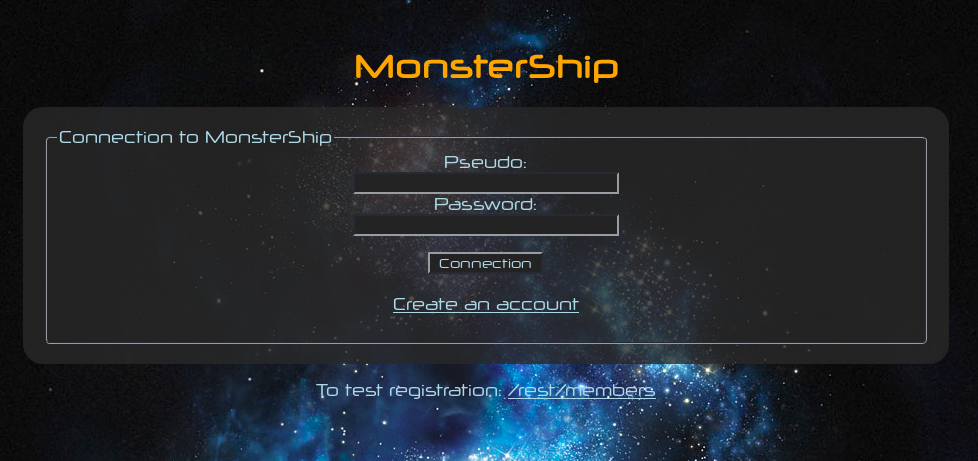
\includegraphics[width=.8\textwidth]{images/connexion.png}
          \caption{Écran de connexion}
          \label{fig:ec_co}
        \end{center}
      \end{figure}
      \begin{figure}[H]
        \begin{center}
          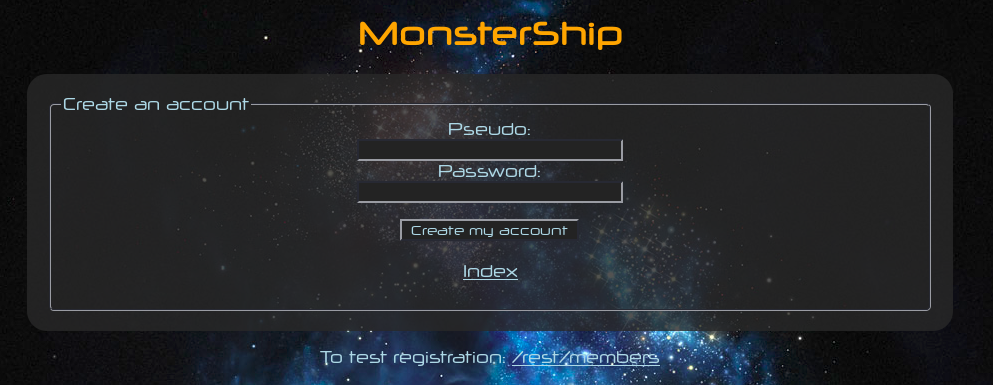
\includegraphics[width=.8\textwidth]{images/inscription.png}
          \caption{Écran d'inscription}
          \label{fig:ec_inc}
        \end{center}
      \end{figure}

    \subsection{Visualisation de la carte et déplacements}
      Une fois l'utilisateur connecté (après une connexion ou une inscription valide), l'utilisateur accède à certaines informations de son vaisseau et à la map de la zone où il se trouve.
      Nous affichons le nom du commander, les coordonnées de son vaisseau, son équipage et le nombre de points d'action qu'il lui reste. Ces informations sont mis à jours dynamiquement à chaque déplacement.
      Pour se déplacer, l'utilisateur doit cliquer sur les cases de la carte en sachant qu'il ne peut se déplacer qu'horizontalement ou verticalement. De même l'affichage de la carte est dynamique.
      \begin{figure}[H]
        \begin{center}
          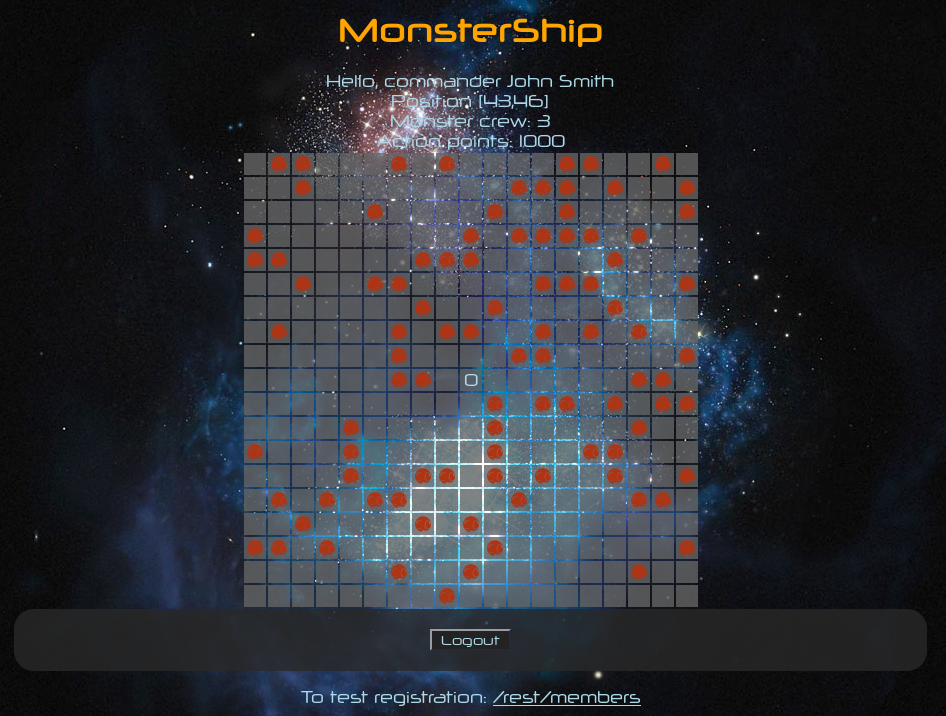
\includegraphics[width=.8\textwidth]{images/home.png}
          \caption{Écran principal du jeu}
          \label{fig:ec_home}
        \end{center}
      \end{figure}

    \subsection{Récolte de monstres}

\chapter{La suite}

  \section{Les fonctionnalités non implémentées}
    Liste des fonctionnalités qui étaient prévus mais non implémentées :
    \begin{itemize}
      \item nous ne pouvons ni abandonner le vaisseau, ni récupérer les vaisseaux abandonnées pour leurs ressources
      \item nous ne pouvons attaquer d'autres joueurs
      \item et les fonctionnalités liées à la gestion du vaisseau :
      \begin{itemize}
        \item ajouter des modules et pouvoir les améliorer
        \item affecter des monstres aux modules
      \end{itemize}
    \end{itemize}

  \section{D'autres idées}

\chapter{Conclusion}

\chapter{Annexes}

  \section{Cahier des charges}
    
\includepdf[pages=1-17]{cahier_des_charges.pdf}
\end{document}
